\chapter{Turn It Up to Eleven: What Is a Knob?}

\epi{A theory with no knobs predicts everything and is almost certainly wrong.\\ A theory with infinitely many knobs predicts nothing and is never wrong.\\ Physics lives in between, counting.}

\section{The amplifier problem}

Imagine you've been handed a black box with a speaker on the front and a row of dials on top. Somebody plays a song in another room, and your job is to make the box reproduce it. If the box has one dial, volume, you'll get the loudness right and nothing else. Add bass and treble and you're doing better. Give it a thirty-band equaliser, a reverb unit, a pitch shifter and a sampler, and you can make it reproduce the song perfectly. You could also make it reproduce any other song, or a dog barking, or the sound of the sea.

That is the whole problem of free parameters in one picture. A box that can only make one sound is either a stunning discovery or useless, depending on whether it's the right sound. A box that can make every sound tells you nothing about the song. Most scientific theories are somewhere in the middle, and how much they tell you depends on where.

\fig{panels}{Four control panels, drawn to scale where possible. The law has one dial. \LCDM's fit to the microwave background has six. Its galaxy modelling has dozens to about a thousand. The string landscape has one dial with $10^{500}$ settings.}


\section{A definition}

Let a theory be a machine $M$ that takes a list of numbers $\boldsymbol\theta=(\theta_1,\dots,\theta_k)$ and returns predictions for a set of observations $\mathbf{d}=(d_1,\dots,d_n)$:
\begin{equation}
\mathbf{d}_{\rm pred}=M(\boldsymbol\theta).
\end{equation}
Some numbers in $\boldsymbol\theta$ are fixed by things outside the problem: the speed of light, Newton's constant, the mass of the proton. Others are not. The theory doesn't say what they are, so you set them by comparing $\mathbf{d}_{\rm pred}$ to the real $\mathbf{d}$ and adjusting. Those are the knobs.

\begin{knobbox}{Knob, defined}
A \textbf{knob} is any number, function or choice in a model whose value is set by looking at the data the model is meant to explain, rather than by the model's own logic or by an independent measurement.
\end{knobbox}

The definition has teeth because of the last clause. If you measure the mass of the electron in a lab and then use it to predict the hydrogen spectrum, the electron mass isn't a knob for the hydrogen problem; it came from elsewhere. If you set it by fitting the hydrogen spectrum, it is. The same number can be a knob in one problem and an input in another. What makes something a knob is where its value came from.

\section{A field guide to knobs}

Knobs come in several species, and part of the fun of this book is learning to spot them in the wild. Here are the ones we'll meet.

\begin{description}[leftmargin=1em,style=nextline]
\item[Global knobs.] One number for the whole universe. The density of dark matter in \LCDM, or the coefficient $\kappa$ in my galaxy law. These are the honest, visible dials on the front panel.
\item[Per-object knobs.] One number \emph{per galaxy}, per cluster or per star. A galaxy's halo mass, its concentration, its distance, its inclination, its stellar mass-to-light ratio $\Upsilon$. These multiply: six per-galaxy knobs over 171 galaxies is 1026 knobs. They are often called \emph{nuisance parameters}, which makes them sound harmless. Some are, if an independent measurement constrains them tightly. Some aren't.
\item[Shape knobs.] The choice of a \emph{function} rather than a number. Do halos follow the NFW profile or the Einasto profile? Is the interpolation between two regimes sharp or gentle? A choice of function hides an infinite number of potential knobs behind a single decision.
\item[Hand terms.] A dependence written in after seeing that the fit fails without it. ``Let the concentration scale as the dark energy density to the third power.'' A hand term is a knob that also confesses something: the model didn't produce this behaviour, so somebody typed it in.
\item[Priors.] Soft knobs. A range or a probability distribution that says how far a knob is allowed to move. Widening a prior is quietly turning a knob's limit stop.
\item[Choices of sample and statistic.] Which galaxies are kept, which data points are cut, which goodness-of-fit number is reported. These are the knobs nobody lists. Good practice is to freeze them in writing \emph{before} looking at the result.
\end{description}

\section{The elephant in the room}

There's a famous story about knobs. In 1953 the young Freeman Dyson travelled to Chicago to show Enrico Fermi a calculation that agreed nicely with Fermi's own measurements. Fermi wasn't impressed. He asked how many arbitrary parameters Dyson had used. Four, said Dyson. Fermi then repeated a remark he attributed to John von Neumann: with four parameters you can fit an elephant, and with five you can make it wiggle its trunk. Dyson took the train home and dropped the project. He told the story half a century later in \emph{Nature}.

In 2010 three physicists, J\"urgen Mayer, Khaled Khairy and Jonathon Howard, took the joke literally. They drew an elephant outline with four complex parameters, which is eight real numbers if you are counting carefully, and used a fifth to wiggle the trunk. It works. The elephant looks like an elephant. The point of the exercise was the same as the point of this book. A fit that looks wonderful may only be telling you how many knobs you had.

\section{Counting with a polynomial}

Here is the elephant in mathematical form. Take $n$ data points $(x_i,y_i)$ with distinct $x_i$. A polynomial of degree $n-1$,
\begin{equation}
p(x)=\sum_{j=0}^{n-1}\theta_j x^j,
\end{equation}
has $k=n$ coefficients. The $n$ equations $p(x_i)=y_i$ form a linear system whose matrix (the Vandermonde matrix) is invertible whenever the $x_i$ are distinct. So there is always exactly one polynomial through all $n$ points. The fit is perfect, $\chi^2=0$, and it means nothing at all, because it would be perfect for any $y_i$ whatever.

We'll see this precise situation in Chapter~5. A recipe called R5 gives every one of 3373 radial shells in 171 galaxies its own dark-matter mass. It has 3373 knobs for 3373 data points. It matches my law with an rms error of $0.0000\dex$. It's the polynomial through all the points, dressed as a halo.

\fig{elephant}{The elephant in miniature. Eight measurements of a straight line with noise. Two knobs (blue) capture the trend. Eight knobs (red) pass through every point exactly and swing wildly in between and beyond. A perfect fit with as many knobs as data points says nothing.}


\section{Goodness of fit, and its blind spot}

The workhorse statistic is chi-squared. For independent Gaussian errors $\sigma_i$,
\begin{equation}
\chi^2(\boldsymbol\theta)=\sum_{i=1}^{n}\frac{\bigl[d_i-M_i(\boldsymbol\theta)\bigr]^2}{\sigma_i^2}.
\end{equation}
Minimise it over the knobs to get $\chi^2_{\min}$. If the model is right and the errors are honest, $\chi^2_{\min}$ should be about the number of \emph{degrees of freedom},
\begin{equation}
\nu=n-k,
\end{equation}
with a scatter of about $\sqrt{2\nu}$. Here is the first place knob-counting enters: every knob you add lowers the expected $\chi^2$ by about one, because it soaks up one dimension of the noise. A model with $k=n$ has $\nu=0$ and fits perfectly whether or not it's true.

In this book I'll often quote a simpler number, the \textbf{rms distance in dex},
\begin{equation}
\mathrm{rms}=\left[\frac1n\sum_{i=1}^{n}\left(\log_{10}g_{{\rm model},i}-\log_{10}g_{{\rm target},i}\right)^2\right]^{1/2},
\end{equation}
because the fried chicken experiment compares a recipe to a target \emph{law} rather than to noisy data, so there are no error bars to divide by. The rms has the same blind spot as $\chi^2$. More knobs always lower it, or at least never raise it on the data used to set them.

\section{Two cures: holdouts and penalties}

There are two standard ways to stop knobs from flattering you.

\textbf{Hold some data out.} Split the sample in two. Turn the knobs on the first half, then grade on the second half without touching anything. A model that has learned something real does about as well on the unseen half. A model that has memorised noise falls apart. In the fried chicken experiment the twelve-knob recipe scored $0.0405\dex$ on the half it was tuned on and $0.0445\dex$ on the half it hadn't seen. That's a small drop, so the recipe generalises. Note, though, that a recipe can generalise beautifully and still be an imitation. Generalising only means the knobs captured a pattern; it doesn't say where the pattern came from.

\fig{holdout}{Why hold data out. Fitting noisy data with more and more knobs always lowers the error on the data used (blue). The error on data held out (red) falls, bottoms out, then climbs as the knobs start fitting noise.}


\textbf{Charge rent for each knob.} Information criteria add a penalty that grows with $k$. The two most common are
\begin{align}
\mathrm{AIC}&=2k-2\ln\mathcal{L}_{\max},\\
\mathrm{BIC}&=k\ln n-2\ln\mathcal{L}_{\max},
\end{align}
where $\mathcal{L}_{\max}$ is the best-fit likelihood (for Gaussian errors, $-2\ln\mathcal{L}=\chi^2$ plus a constant). Lower is better. AIC charges 2 per knob. BIC charges $\ln n$ per knob, which for the fried chicken sample of $n=3373$ points is $8.1$.

\begin{knobbox}{The rent, in numbers}
With $n=3373$ points, BIC's penalty $k\ln n$ is
\begin{center}
\begin{tabular}{lrr}
\toprule
model & $k$ & penalty\\
\midrule
one-knob law & 1 & 8.1\\
twelve-knob recipe & 12 & 97.5\\
fourteen-knob recipe & 14 & 113.7\\
per-galaxy recipe & 1026 & 8334.8\\
\bottomrule
\end{tabular}
\end{center}
A per-galaxy model must beat the one-knob law's $\chi^2$ by more than eight thousand just to break even. Sometimes it does. In Chapter~8 we'll meet a case where cored halos fitted galaxy by galaxy beat my law on observed rotation curves even after paying this rent.
\end{knobbox}

\fig{bic_rent}{Rent per knob. BIC charges $\ln n\approx8.1$ per knob on the fried chicken sample, AIC charges 2. The recipes of Part~II are marked.}


\section{The Occam factor}

The deepest version of knob rent comes from Bayesian probability, and it has a lovely geometric meaning. The \emph{evidence} for a model is the probability of the data averaged over everything the model could have said before seeing it:
\begin{equation}
\mathcal{Z}=\int \mathcal{L}(\boldsymbol\theta)\,\pi(\boldsymbol\theta)\,d^k\theta,
\end{equation}
where $\pi$ is the prior, the range of knob settings the model allowed in advance. Comparing two models, the ratio $\mathcal{Z}_1/\mathcal{Z}_2$ (the Bayes factor) says how much the data shift the odds between them.

\begin{mathbox}{Where the Occam factor comes from}
Take one knob with a flat prior of width $\Delta$, so $\pi=1/\Delta$ inside the range. Suppose the likelihood is a Gaussian bump of width $\sigma_{\rm post}$ around its peak $\mathcal{L}_{\max}$, well inside the range. Then
\[
\mathcal{Z}=\frac{1}{\Delta}\int\mathcal{L}_{\max}\,e^{-(\theta-\hat\theta)^2/2\sigma_{\rm post}^2}\,d\theta
=\mathcal{L}_{\max}\times\underbrace{\frac{\sqrt{2\pi}\,\sigma_{\rm post}}{\Delta}}_{\text{Occam factor}}.
\]
The Occam factor is the fraction of the prior range that survives the data. With $k$ independent knobs it is the product of $k$ such fractions. Every knob whose range the data squeeze by a factor of 100 costs a factor of about 100 in evidence. A model only gets that back if its best fit is that much better.
\end{mathbox}

\begin{figure}[h]
\centering
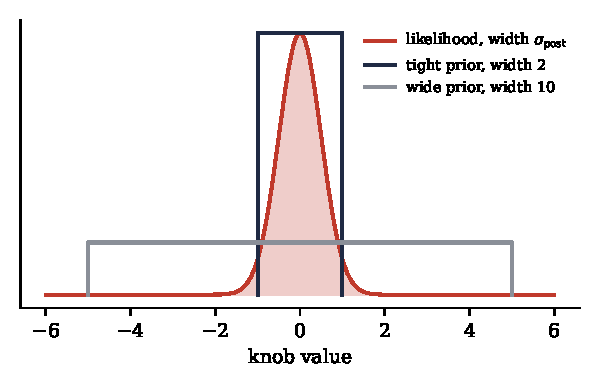
\includegraphics[width=0.85\linewidth]{figures/occam.pdf}
\caption{The Occam factor. The same likelihood (red) under a tight prior and a wide prior. Spreading the prior over a wider range of knob settings lowers its height everywhere, including where the data actually are. A model that ``could have said anything'' is penalised for that freedom automatically.}
\end{figure}

This is Occam's razor with numbers in it. It doesn't say simple models are true. It says a model that could have accommodated a wide range of outcomes gets less credit when the actual outcome turns up, because it spread its bets.

\section{Knobs measured in bits}

There's a neat way to put all knobs on one scale. A knob whose prior range is $\Delta$ and whose data-allowed width is $\sigma$ carries about
\begin{equation}
I=\log_2\frac{\Delta}{\sigma}\ \text{bits}
\end{equation}
of information extracted from the data. That's the number of yes-or-no questions the data had to answer to pin it down. It's also, roughly, minus the base-2 logarithm of the Occam factor.

Take my one galaxy knob, $\kappa$. Suppose before looking you'd have allowed anything from $0.1$ to $10$, a range of 2 dex, and the data pin it to about 5 per cent, or $0.021\dex$. Then
\[
I_\kappa=\log_2\frac{2}{0.0212}\approx6.6\ \text{bits}.
\]
Six and a half yes-or-no questions. Keep that number in mind. We'll compare it with $\log_2(10^{500})\approx1661$ bits in Part~III.

\fig{bits_per_knob}{Information in a knob, $\log_2$ of how much the data shrink its allowed range. Every factor of two is one bit.}


\section{Knobs at the bounds}

One more diagnostic will matter a great deal in Part~II. When you tune a model inside sensible prior ranges and a knob runs to the edge of its range and stays there, the model is telling you something. It wants to go further than its physics allows. A fit with several knobs pinned at their limits isn't a model behaving naturally; it's a model being stretched.

The fried chicken paper reports, for every recipe, how many knobs sit at their bounds. The twelve-knob recipe has three. The ``complete'' recipe of Chapter~7 has seven, against a limit of three set in advance. When half of 171 galaxies push their halo concentration to the same lower edge, that's not scatter. It's a population asking for a different kind of halo.

\section{Freeze first, then turn}

The last knob is the most dangerous because it's invisible: the freedom to decide \emph{after} seeing the results what counts as success. Physicists call this the garden of forking paths, or, less politely, moving the goalposts. The cure is to write the targets down, date them and commit them before the first number is computed. The programme behind this book does this for every calculation, which it calls a \emph{lane}. Each lane commits its criteria to a public repository before any script exists. It also runs a deliberately broken twin, called MUTATE, which must fail; if it passes, the test can't tell right from wrong. Failures are published under the label frozen in advance.

The fried chicken paper's targets were frozen before any recipe was cooked:
\begin{itemize}
\item \textbf{E1}: pooled rms distance to the law at most $0.02\dex$;
\item \textbf{E2}: 95th percentile of per-galaxy rms at most $0.04\dex$;
\item \textbf{E3}: no half-dex bin in $\gbar$ off by more than $0.02\dex$;
\item \textbf{E4}: the fitted scale must vary with the dark energy density as $d\ln a/d\ln\rhoDE=0.50\pm0.05$;
\item \textbf{E5}: the scale's change with redshift must sit inside the law's predicted band.
\end{itemize}
Recipes were added later at my request, and every one of them is disclosed as a dated amendment. The targets never moved.

\section{The rules of knob accounting}

Here are the rules this book will follow, for every theory, including mine.

\begin{enumerate}
\item \textbf{Count every number set by the data being explained.} Global, per-object, hand terms, all of them.
\item \textbf{Count a hand term twice}: once as a knob, and once as a confession that the model didn't produce the behaviour.
\item \textbf{Report knobs at their bounds.} A stretched knob is a model asking for different physics.
\item \textbf{Hold data out.} A fit on unseen data counts for more than a fit on the data used for tuning.
\item \textbf{An imitation proves freedom, not truth.} If a model was tuned to reproduce a target, matching the target tells you the model was flexible enough. It does not tell you the target is real, and it does not tell you the model is right.
\item \textbf{Fewer knobs is a virtue, not a verdict.} A one-knob theory can be wrong, and a hundred-knob theory can be right. Knob-counting tells you how much each theory has risked, and the data decide the rest.
\end{enumerate}

Rule 6 matters most, and it's the one most often broken in popular writing about cosmology, in both directions. Let's go and look at the knobs on the most successful theory in cosmology, and give it the credit it has earned.
